\chapter{Analisis}
\label{chap:analisis}
Bab Analisis berisi pemahaman lebih lanjut berdasarkan teori-teori yang sudah dijelaskan dari Bab Landasan Teori. Pada bagian ini akan dijelaskan analisis lebih lanjut terhadap masalah yang sudah dijelaskan pada latar belakang. Teori yang sudah dijelaskan sebelumnya pada Landasan Teori akan diberi contoh permasalahan dan cara penyelesaiannya. 

\section{Analisis Masalah}
Penelitian \textit{"Analisis Kesuksesan Film Menggunakan Data Mining"} merupakan penelitian yang akan menggunakan \textit{dataset} yang berasal dari \textit{Kaggle} \footnote{PromptCloud, (2017)\textit{"IMDB data from 2006 to 2016"} https://www.kaggle.com/PromptCloudHQ/imdb-data . 18 April 2020.}. \textit{Dataset} yang digunakan adalah kumpulan film populer dari tahun 2006 sampai 2016. Terdapat informasi yang terkait dengan sebuah film seperti judul, aktor, \textit{genre}, \textit{rating} dan lain-lain. Penjelasan lebih lengkap mengenai \textit{dataset} dan proses penelitian akan dibahas pada Bab 4.

Berdasarkan Landasan Teori yang dijelaskan pada Bab \ref{chap:teori} mengenai tahap \textit{Data Mining}, penelitian ini akan menerapkan langkah-langkah \textit{Data Mining} untuk mendapatkan pola yang menarik. Pola yang menarik adalah informasi yang dapat menjawab masalah yang sudah dijelaskan pada bagian Latar Belakang. Penelitian ini akan menghasilkan pengujian faktor yang mempengaruhi kesuksesan film dengan menggunakan \textit{Data Mining} dan \textit{Machine Learning}. 

Penelitian ini akan membuat beberapa program terpisah yang akan memproses \textit{dataset} yang sudah dipilih. Program yang dihasilkan bukan suatu program dengan antarmuka yang bisa menerima \textit{input} dan mengeluarkan \textit{output}, Tetapi hasil eksperimen berdasarkan \textit{dataset} dengan menerapkan langkah \textit{data mining} dan gambar visualisasi data. Penelitian ini akan menggunakan bahasa pemrograman \textit{Python} dan memanfaatkan beberapa  \textit{library} pada \textit{Python} yang akan membantu penelitian pada Bab 4. Berikut adalah kumpulan \textit{library} yang digunakan untuk penelitian : 

\begin{itemize}
\item \textit{Pandas} : melakukan operasi pemrosesan analisis data pada tabel bernama \textit{DataFrame}
\item \textit{NumPy}  : melakukan beberapa fungsi hitung matematika pada kumpulan \textit{Array} 
\item \textit{Matplotlib} : melakukan analisis dalam bentuk visualisasi data 
\item \textit{Seaborn} : melakukan visualisasi data dan menyediakan fungsi kompleks yang tidak dimiliki \textit{matplotlib}
\item \textit{Scikit-learn} : melakukan analisis data dengan melakukan algoritma pada \textit{Machine Learning}
\item \textit{Pickle} : menyimpan model / algoritma \textit{Machine Learning} yang sudah diproses sehingga tidak perlu melakukan \textit{training} untuk melakukan prediksi 
\item \textit{os}     : melakukan fungsi yang dapat berkomunikasi dengan sistem operasi seperti membaca dan menyimpan data 
\item \textit{shutil} : melakukan operasi manipulasi dan memproses \textit{file} pada sistem operasi
\item \textit{requests} : melakukan HTTP \textit{Request} untuk	melakukan pemanggilan API mengambil data yang tambahan yang akan digunakan saat penelitian 
\item \textit{json}   : melakukan konversi JSON (sintaks untuk menyimpan data) secara universal dan mengubah menjadi struktur data di \textit{Python} 
\end{itemize}

\section{Tahap Pengerjaan Penelitian}
Berdasarkan penjelasan pada bagian sebelumnya tentang Analisis Masalah, dibuat rencana yang berisi langkah-langkah yang dilakukan selama analisis data pada Bab 4. Berdasarkan ilustrasi gambar proses \textit{Data Mining} pada Landasan Teori Bab \ref{chap:teori}, proses \textit{Data Mining} dijelaskan sebagai sebuah siklus. Hasil sebuah siklus dapat dijadikan pengantar analisis pada siklus selanjutnya. Penelitian ini dibagi menjadi 3 siklus iterasi yaitu : 

\begin{itemize}
\item Analisis Data Utama
\item Analisis Data Tambahan IMDB
\item Analisis Data Media Sosial
\end{itemize} 

\subsection{Analisis Data Utama}
Penelitian dimulai dengan menggunakan \textit{dataset} yang sudah dipilih. Pada analisis tahap ini akan melakukan \textit{Data Cleaning} , \textit{Data Selection}, analisis visualisasi dan percobaan prediksi kesuksesan yaitu \textit{revenue} / pendapatan kotor. Percobaan prediksi akan menggunakan 2 algoritma regresi dan membandingkan performa yang dihasilkan. 

 
Hasil prediksi regresi pada data utama akan dilanjutkan dengan analisis yang lebih detail. Akan dilakukan analisis \textit{clustering} untuk mengelompokkan film dengan karakteristik yang sama. Setiap film memiliki sifat berbeda dalam mendefinisikan kesuksesannya. Fitur yang menjadi penentu kelompoknya adalah aktor dan \textit{genre}.

\subsection{Analisis Data Tambahan IMDB} 
Hasil dan performa analisis data utama akan digunakan sebagai latar belakang bagi analisis data tambahan. Pada tahap ini akan dilakukan pengumpulan data tambahan. Tahap pengumpulan data tambahan akan dilakukan dengan \textit{Scraping} dan mengakses API dari situs IMDB. Data tambahan akan diintegrasikan ke \textit{dataset} awal sesuai dengan tahap \textit{Data Mining} yaitu \textit{Data Integration}. Data tambahan akan dianalisis sesuai dengan tahap sebelumnya untuk menguji apakah data tambahan dapat membantu meningkatkan akurasi / pengaruh dalam memprediksi kesuksesan film.


Tahap \textit{Data Transformation} juga dilakukan dimana kolom pada \textit{dataset} utama dapat digabung dengan kolom tambahan sehingga mendapatkan kolom baru yang dapat dianalisis. Prediksi kolom baru akan dilakukan untuk mengetahui apakah terdapat faktor yang memiliki korelasi yang tinggi dengan apa yang ingin diprediksi.


\subsection{Analisis Data Sosial Media}
Penonton / penikmat film juga memiliki peran penting dalam menentukan kesuksesan film. \textit{Analisis} data yang sudah dilakukan sebelumnya hanya terikat dengan informasi yang melekat pada filmnya saja seperti aktor, \textit{genre}, \textit{budget} dan \textit{rating}. Media sosial merupakan salah satu cara pembuat film untuk mempromosikan hasil karyanya kepada penonton dengan merilis seperti \textit{trailer} dan poster. Pada analisis data media sosial akan dilakukan pengumpulan data seperti \textit{Youtube} dan \textit{Instagram}. 

Data media sosial tambahan yang sudah dikumpulkan akan dianalisis lebih lanjut sesuai dengan tahap \textit{Data Mining}. Pengujian  akan dilakukan apakah data media sosial dapat membantu meningkatkan akurasi prediksi kesuksesan film. Data media sosial juga akan dianalisis apakah memiliki korelasi yang tinggi dengan pendapatan. 

\section{Analisis Penerapan Data Cleaning}
Penjelasan Bab \ref{chap:teori} Landasan Teori mengenai \textit{Data cleaning} menyebutkan bahwa terdapat beberapa jenis data kotor. Data yang tidak sesuai dan \textit{missing value} adalah salah satu masalah \textit{Data Cleaning}. Cara mengatasi hal tersebut adalah dengan mengabaikan data tersebut. Berikut adalah contoh data tabular \textit{dataset} yang terdapat data kotor didalamnya.


\begin{figure}[H]
	\centering  
	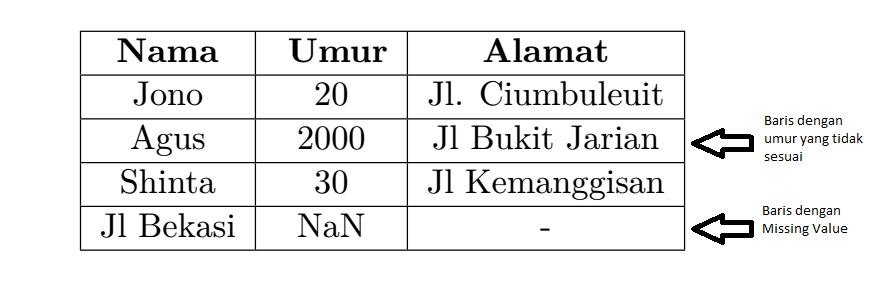
\includegraphics[scale=0.7]{bab4/tabeldatacleaning}   
	\caption{Contoh dataset yang memiliki data kotor}
	\label{fig:tabeldatacleaning} 
\end{figure} 


berdasarkan Gambar \ref{fig:tabeldatacleaning} yang sudah ditunjuk panah, terdapat baris yang tidak sesuai seperti baris terakhir yang pada kolom 'Nama' tidak terisi yang sesuai. Baris ketiga juga merupakan data kotor dikarenakan isi pada kolom 'Umur' tidak sesuai dengan rentang umur manusia pada umumnya sehingga data tersebut harus diabaikan. 

\textit{Library Pandas} menyediakan fungsi untuk mendeteksi baris pada data tabel yang terdapat nilai NaN pada kolomnya. Gambar \ref{fig:code_analisisdatacleaning} adalah potongan kode untuk membaca \textit{DataFrame} dari sebuah file lalu menghilangkan baris yang NaN.
%
%% source code for data cleaning
%\begin{lstlisting}[float,language=Python, caption=Library Data Cleaning]
%import pandas as pd 
%
%# read dataset 
%dataset = pd.read_csv('table.csv') 
%
%#remove row with NaN in dataset 
%dataset = dataset.dropna()
%\end{lstlisting}


\begin{figure}[H]
	\centering  
	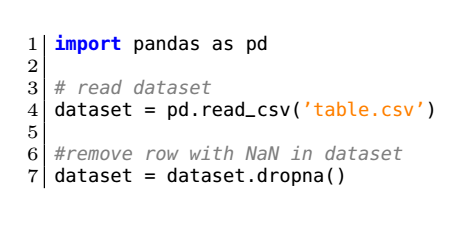
\includegraphics[scale=0.7]{bab4/code_analisisdatacleaning}   
	\caption{Kode analisis data cleaning}
	\label{fig:code_analisisdatacleaning} 
\end{figure} 



\section{Analisis Penerapan Data Transformation}
Berdasarkan penjelasan Bab \ref{chap:teori} Landasan Teori tentang \textit{Data Transformation}, beberapa  cara yang dapat dilakukan adalah \textit{Attribute Construction} dan \textit{Normalization}. Akan diberikan beberapa contoh penerapan \textit{Data Transformation}. Berikut adalah contoh \textit{dataset} dari penjualan barang pada toko oleh-oleh yang akan dibuat kolom baru.

\subsection{Attribute Construction}

\begin{table}[H]
\caption{Tabel contoh yang perlu diubah}
\centering
\begin{tabular}{|c|c|c|c|}
\hline 
\textbf{Barang} & \textbf{Harga Satuan} & \textbf{Jumlah Terjual} & \textbf{Total Terjual} \\ 
\hline 
Slondok & 2000 & 20 & 40000 \\ 
\hline 
Keripik Singkong & 2500 & 5 & 12500 \\ 
\hline 
Getuk & 10000 & 1 & 10000 \\ 
\hline 
\end{tabular} 
\label{tab:TabelSebelumDataTransformation}
\end{table}

Tabel \ref{tab:TabelSebelumDataTransformation} menunjukkan hasil penjualan dari tiap barang. Dalam menentukan barang mana yang menguntungkan ternyata dibutuhkan persenan kontribusi keuntungan dari tiap item. Dibutuhkan kolom baru dari tiap barang untuk menghitung kontribusi. Kontribusi dapat dihitung menggunakan rumus di bawah.

\begin{equation}
  Kontribusi Barang(i) = \frac{Total Penjualan Barang (i)}{Total Penjualan Semua Barang}
  \label{eqref:RumusKontribusi}
\end{equation}

Persamaan \ref{eqref:RumusKontribusi} dapat digunakan untuk menghitung kontribusi setiap barang. Total penjualan semua barang adalah $Rp.62500$. Tabel \ref{tab:TabelSesudahDataTransformation}  adalah hasil tabel yang baru setelah ditambahkan kolom baru bernama kontribusi.

\begin{table}[H]
\caption{Tabel dengan kolom baru setelah \textit{Data Transformation}}
\centering
\begin{tabular}{|c|c|c|c|c|}
  \hline 
  \textbf{Nama Barang} & \textbf{Harga Satuan} &\textbf{ Jumlah Terjual} & \textbf{Total Penjualan} & \textbf{Kontribusi }\\ 
  \hline 
  Slondok & 2000 & 20 & 40000 & 0.64 \\ 
  \hline 
  Keripik Singkong & 2500 & 5 & 12500 & 0.2 \\ 
  \hline 
  Getuk & 10000 & 1 & 10000 & 0.16 \\ 
  \hline 
  \end{tabular}   
  \label{tab:TabelSesudahDataTransformation}
\end{table} 

Manipulasi sebuah data tabel dapat dilakukan oleh \textit{Library Pandas}. Gambar \ref{fig:code_analisistransformation_attribute} adalah kode implementasi menggunakan bahasa \textit{Python} untuk melakukan \textit{Data Transformation}.


\begin{figure}[H]
	\centering  
	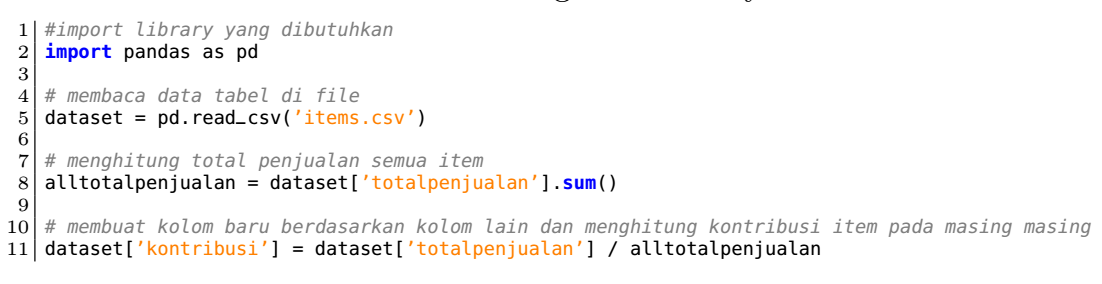
\includegraphics[scale=0.5]{bab4/code_analisistransformation_attribute}   
	\caption{Kode contoh Attribute Construction}
	\label{fig:code_analisistransformation_attribute} 
\end{figure} 

\subsection{Normalization}

Penjelasan mengenai \textit{Normalization} pada Bab 2 yaitu salah satunya adalah dengan menggunakan \textit{MinMaxNormalization}. Persamaan \eqref{eqref:minmaxscaler} adalah rumus yang dapat digunakan untuk melakukan normalisasi.

\begin{equation}
z = \frac{x - min(x)}{max(x) - min(x)} 
\label{eqref:minmaxscaler}
\end{equation}

Persamaan \eqref{eqref:minmaxscaler} di atas merupakan cara mengubah sebuah angka dari kumpulan data dalam bentuk yang sudah dinormalisasi. $x$ adalah nilai yang ingin rubah dalam bentuk normalisasi. $min(x)$ adalah nilai terkecil dalam kumpulan data dan $max(x)$ adalah nilai terbesar. Selanjutnya akan diberikan contoh dalam mengubah kumpulan dalam bentuk yang sudah dinormalisasi dalam bentuk tabel.

\begin{table}[H]
\caption{Tabel Dataset yang ingin dinormalisasi} 
\centering
\begin{tabular}{|c|c|}
\hline 
lamabelajar & nilai \\ 
\hline 
2 & 90 \\ 
\hline 
4 & 70 \\ 
\hline 
6 & 86 \\ 
\hline 
3.5 & 85 \\ 
\hline 
\end{tabular} 
\label{tab:tabelprenormalisasi}
\end{table}

Tabel \ref{tab:tabelprenormalisasi} di atas merupakan tabel performa siswa yang akan dianalisis lebih lanjut sehingga perlu dilakukan normalisasi. Berikut adalah hasil tabel setelah dinormalisasi menggunakan \textit{MinMaxNormalization} berdasarkan persamaan \eqref{eqref:minmaxscaler}. 

\begin{table}[H]
\caption{Tabel dataset setelah dinormalisasi}
\centering
\begin{tabular}{|c|c|c|c|}
\hline 
Lama Belajar & Nilai & Norm Lama Belajar & Norm Nilai \\ 
\hline 
2 & 90 & 0 & 1 \\ 
\hline 
4 & 70 & 0.5 & 0 \\ 
\hline 
6 & 86 & 1 & 0.8 \\ 
\hline 
3.5 & 85 & 0.375 & 0.75 \\ 
\hline 
\end{tabular} 
\label{tab:tabelposnormalisasi}
\end{table}

Tabel \ref{tab:tabelposnormalisasi} di atas merupakan hasil tabel \textit{dataset} setelah dinormalisasi. Pada kolom 'Norm Lama Belajar' dan 'Norm Nilai' adalah nilai setelah sudah dirubah. \textit{Normalization} dapat dilakukan sebelum tahap pemodelan \textit{Machine Learning}. \textit{Library Scikit Learn} pada \textit{Python} menyediakan fungsi untuk mengonversi kumpulan nilai pada tabel dalam bentuk yang sudah dinormalisasi. Gambar \ref{fig:code_analisistransformation_normalization} adalah contoh potongan kode dalam melakukan normalisasi.


\begin{figure}[H]
	\centering  
	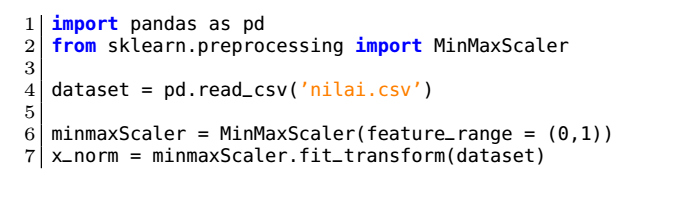
\includegraphics[scale=0.7]{bab4/code_analisistransformation_normalization}   
	\caption{Kode contoh \textit{Normalization}}
	\label{fig:code_analisistransformation_normalization} 
\end{figure} 


\section{Analisis Penerapan Data Integration}
Salah satu cara yang dapat dilakukan dalam melakukan \textit{Data Integration} adalah penggabungan 2 tabel menggunakan operasi \textit{join} seperti pada basis data. Berikut terdapat 2 tabel terpisah yang memiliki relasi.

\begin{table}[H]
\caption{Tabel kumpulan buku}
\centering
\begin{tabular}{|c|c|c|}
\hline 
ID\textunderscore Buku & Judul Buku & Nama Pengarang\\ 
\hline 
1 & Pengantar Basis Data & Bill Gates \\ 
\hline 
2 & Pemrograman Dasar & Bill Gates \\ 
\hline 
3 & Terampil Memasak & Gordon Ramsey \\ 
\hline 
\end{tabular} 
\label{tab:TabelBuku}
\end{table}

\begin{table}[H]
\caption{Tabel pengarang}
\centering
\begin{tabular}{|c|c|}
\hline 
Nama Pengarang & Kota Kelahiran \\ 
\hline 
 Bill Gates & Bekasi\\ 
\hline 
Gordon Ramsey & Bandung\\ 
\hline 
\end{tabular} 
\label{tab:TabelPengarang}
\end{table}

Tabel \ref{tab:TabelBuku} dan \ref{tab:TabelPengarang} dapat digabung agar sebuah buku dapat mengetahui kota asal pengarangnya. Tabel buku berhubungan dengan tabel pengarang karena tabel buku memiliki kolom "Nama Pengarang" untuk mengetahui data pengarang. Berikut adalah tabel \ref{tab:TabelJoinBukuPengarang} yang sudah tergabung.

\begin{table}[H]
\caption{Tabel buku dan pengarang sudah tergabung}
\centering
\begin{tabular}{|c|c|c|c|}
\hline 
ID\textunderscore Buku& Nama Buku & Nama Pengarang & Kota kelahiran \\ 
\hline 
1 & Pengantar Basis Data & Bill Gates & Bekasi \\ 
\hline 
2 & Pemrograman Dasar & Bill Gates & Bekasi \\ 
\hline 
3 & Terampil Memasak & Gordon Ramsey & Bandung \\ 
\hline 
\end{tabular} 
\label{tab:TabelJoinBukuPengarang}
\end{table}

\textit{Library Pandas} pada \textit{Python} dapat digunakan untuk dilakukan untuk melakukan operasi \textit{join}. Berikut adalah potongan contoh kode pada \textit{Python} untuk melakukan operasi \textit{merge} pada Gambar \ref{fig:code_analisisintegration_merge}.


\begin{figure}[H]
	\centering  
	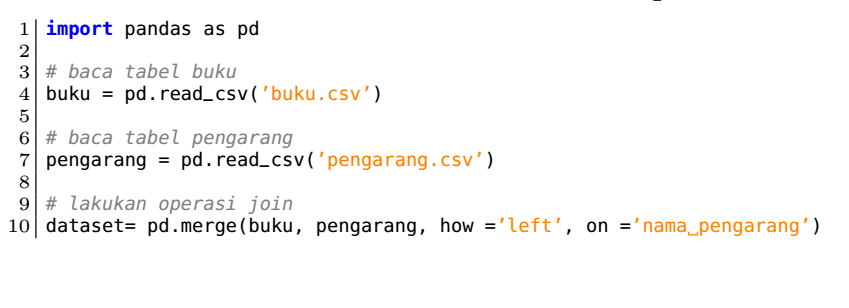
\includegraphics[scale=0.7]{bab4/code_analisisintegration_merge}   
	\caption{Kode contoh \textit{integration}}
	\label{fig:code_analisisintegration_merge} 
\end{figure} 



\section{Analisis Penerapan Data Selection}
Berdasarkan penjelasan pada Bab \ref{chap:teori} mengenai \textit{Data Selection}, \textit{feature selection} adalah cara untuk menentukan fitur sebelum dimodelkan dengan \textit{machine learning}. \textit{Pearson correlation} adalah salah satu teknik untuk menguji korelasi antara 2 fitur. Akan diberikan ilustrasi dalam menentukan / memilih kolom yang memiliki korelasi kuat. Berikut adalah sebuah contoh sederhana dalam memilih kolom yang tepat untuk analisis. Diberikan contoh sebuah tabel penelitian belajar siswa.


\begin{table}[H]
\caption{Tabel data performa belajar siswa}
\centering
\begin{tabular}{|c|c|c|}
\hline 
Lama Belajar dalam Jam & Jam memulai Belajar & Nilai Ujian \\ 
\hline 
2 & 12 & 50 \\ 
\hline 
3 & 10 & 65 \\ 
\hline 
4 & 11 & 70 \\ 
\hline 
\end{tabular} 

\label{tab:TabelDatasetSelection}
\end{table}

Berdasarkan Tabel \ref{tab:TabelDatasetSelection}, ingin dilakukan analisis untuk mengetahui apa yang mempengaruhi performa siswa khususnya dalam memperoleh nilai yang baik. Untuk menemukan kolom / fitur yang berpengaruh, dilakukan perhitungan menggunakan \textit{pearson correlation} untuk membandingkan antara kolom lama belajar dan jam memulai belajar. Berikut adalah hasil perhitungan \textit{pearson correlation}.

\begin{table}[H]
 \caption{Tabel hasil perhitungan pearson}
\centering
\begin{tabular}{|c|c|}
 \hline 
 Pearson (Lama Belajar , Nilai) & Pearson (Jam Mulai , Nilai) \\ 
 \hline 
 0.96 & -0.72 \\ 
 \hline 
 \end{tabular}  
 \label{tab:TabelHasilPearson}
\end{table}

Tabel \ref{tab:TabelHasilPearson} di atas merupakan hasil perhitungan \textit{pearson correlation}. Nilai korelasi antara kolom lama belajar dan hasil nilai memiliki nilai $0.96$. Nilai tersebut memiliki korelasi positif yang kuat. Nilai korelasi positif yang tinggi mendekati $1.0$ menejelaskan bahwa semakin banyak waktu belajar yang dilakukan siswa, maka semakin tinggi kemungkinan siswa untuk mendapatkan nilai yang bagus. Kolom jam mulai dan nilai memiliki korelasi negatif. Berdasarkan itu juga dapat dimaknai bahwa semakin malam siswa belajar maka semakin menurun nilai yang diperoleh. Dapat disimpulkan untuk meningkatkan kemungkinan siswa mendapat nilai bagus adalah dengan meningkatkan frekuensi belajar untuk menguasai materi yang diuji.


\textit{Library Sci Py} pada \textit{Python} menyediakan fungsi \textit{pearson} untuk menghitung korelasi antara 2 kolom nilai. Fungsi \textit{pearsonr(colA , colB)} menerima 2 \textit{input} berupa kolom pertama dan kolom kedua. Gambar \ref{fig:code_analisisdataselection_pearson} adalah potongan kode untuk menghitung korelasi.



\begin{figure}[H]
	\centering  
	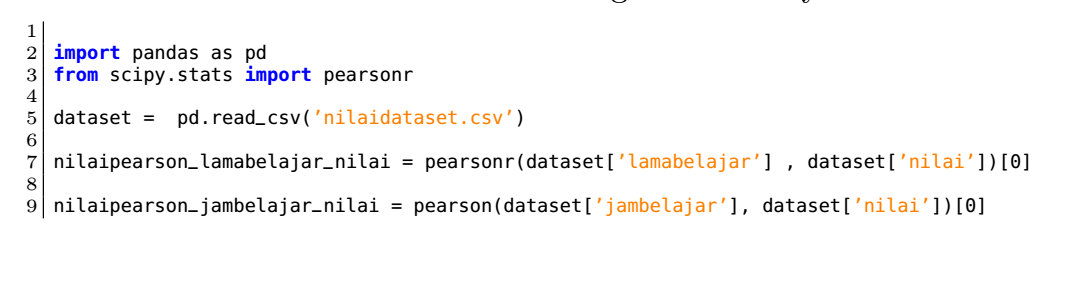
\includegraphics[scale=0.6]{bab4/code_analisisdataselection_pearson}   
	\caption{Kode contoh \textit{pearson correlation}}
	\label{fig:code_analisisdataselection_pearson} 
\end{figure} 



\section{Analisis Penerapan Linear Regression}
\textit{Linear regression} adalah algoritma untuk melakukan prediksi data kontinu dengan menghasilkan persamaan \textit{linear}. Akan dilakukan contoh perhitungan menggunakan \textit{linear regression}. Terdapat \textit{dataset} dengan 2 variabel yaitu suhu ruangan dan jumlah cacat produksi. Diberikan sebuah \textit{dataset} contoh regresi.

\begin{table}[H]
\caption{Tabel dataset regresi }
\centering
\begin{tabular}{|c|c|}
\hline 
Biaya Promosi (X) & Volume Penjualan (Y) \\ 
\hline 
12 & 56 \\ 
\hline 
14 & 62 \\ 
\hline 
13 & 60 \\ 
\hline 
12 & 61 \\ 
\hline 
15 & 65 \\ 
\hline 
13 & 66 \\ 
\hline 
14 & 60 \\ 
\hline 
15 & 63 \\ 
\hline 
13 & 65 \\ 
\hline 
14 & 62 \\ 
\hline 
\end{tabular} 
\label{tab:dataset}
\end{table}

Biaya promosi pada Tabel \ref{tab:dataset} merupakan variabel prediktor / independen (X). Volume penjualan pada Tabel \ref{tab:dataset} merupakan variabel dependen / respon (Y). Tujuan \textit{linear regression} adalah memprediksi volume penjualan berdasarkan biaya promosi yang dikeluarkan. Menggunakan persamaan \textit{linear regression}, maka kita harus mencari a (konstanta) dan b(koefisien) pada persamaan \ref{eqref:linearregression}. Berikut adalah tabel perhitungan $\sum y$  , $\sum x^2$ , $\sum xy$ , $(\sum x)^2$ pada Tabel \ref{tab:konstantakoefisienlinear}.

\begin{table}[H]
\caption{ Perhitungan komponen konstanta dan koefisien}
\centering
\begin{tabular}{|c|c|c|c|c|}
\hline 
no & x & y & $x^2$ & xy \\ 
\hline 
1 & 12 & 56 & 144 & 672 \\ 
\hline 
2 & 14 & 62 & 196 & 868 \\ 
\hline 
3 & 13 & 60 & 169 & 780 \\ 
\hline 
4 & 12 & 61 & 144 & 732 \\ 
\hline 
5 & 15 & 65 & 225 & 975 \\ 
\hline 
6 & 13 & 66 & 169 & 858 \\ 
\hline 
7 & 14 & 60 & 196 & 840 \\ 
\hline 
8 & 15 & 63 & 225 & 945 \\ 
\hline 
9 & 13 & 65 & 169 & 845 \\ 
\hline 
10 & 14 & 62 & 196 & 868 \\ 
\hline 
$\sum $ & 135 & 620 & 1833 & 8383 \\ 
\hline 
\end{tabular} 
\label{tab:konstantakoefisienlinear}
\end{table} 

Setelah menghitung komponen untuk konstanta dan koefisien, maka akan diterapkan pada rumus konstanta dan koefisien sesuai Persamaan \ref{eqref:koefisienregresi}.

\begin{equation}
 a = \frac{(620)(1833) - (135)(8383)}{10(1833) -18255 }  = 45.29
 \label{eqref:konstantacontoh}
\end{equation}
\begin{equation}
 b = \frac{10(8383) - (135)(620)}{10(1833) -18255 } = 1.24 
 \label{eqref:koefisiencontoh}
\end{equation}

Koefisien dan konstanta yang diperoleh pada Persamaan \ref{eqref:koefisiencontoh} dan \ref{eqref:konstantacontoh}  dapat diterapkan pada rumus \textit{linear regression} pada Persamaan \ref{eqref:linearregression}. Persamaan  \textit{linear regression} dapat dibuat.
 
\begin{equation}
  Y = 45.29 + 1.24X
  \label{eqref:contohpersamaanlinear}
\end{equation}
Menggunakan Persamaan \ref{eqref:contohpersamaanlinear} yang sudah diperoleh, maka prediksi volume penjualan menggunakan \textit{linear regression} dapat dihitung menggunakan biaya promosi. Berikut adalah tabel perbandingan antara volume penjualan asli (Y) dan volume penjualan prediksi \textit{linear regression} (\^{Y}) pada Tabel \ref{tab:perbandinganlinearregression}.



\begin{table}[H]
\caption{Tabel perbandingan volume penjualan prediksi dan volume penjualan asli}
\centering
\begin{tabular}{|c|c|c|}
\hline 
Biaya Promosi (X) & Volume Penjualan (Y) & Volume Penjualan Prediksi (\^{Y}) \\ 
\hline 
12 & 56 & 60.14 \\ 
\hline 
14 & 62 & 62.62 \\ 
\hline 
13 & 60 & 61.38 \\ 
\hline 
12 & 61 & 60.14 \\ 
\hline 
15 & 65 & 63.86 \\ 
\hline 
13 & 66 & 61.38 \\ 
\hline 
14 & 60 & 62.61 \\ 
\hline 
15 & 63 & 63.86 \\ 
\hline 
13 & 65 & 61.38 \\ 
\hline 
14 & 62 & 62.61 \\ 
\hline 
\end{tabular} 
\label{tab:perbandinganlinearregression}
\end{table}

\textit{Library Scikit learn} pada \textit{Python} menyediakan fungsi untuk melakukan prediksi menggunakan algoritma \textit{Linear Regression}. Kelas \textit{Linear Regression} tersedia di \textit{package sklearn.model}. Pemodelan \textit{linear regression} menerima \textit{input} kolom \textit{predictor} (Biaya Promosi) dan kolom \textit{response} (Volume Penjualan). Gambar \ref{fig:code_analisislinearregression} adalah potongan kode untuk melakukan \textit{Linear Regression}.


\begin{figure}[H]
	\centering  
	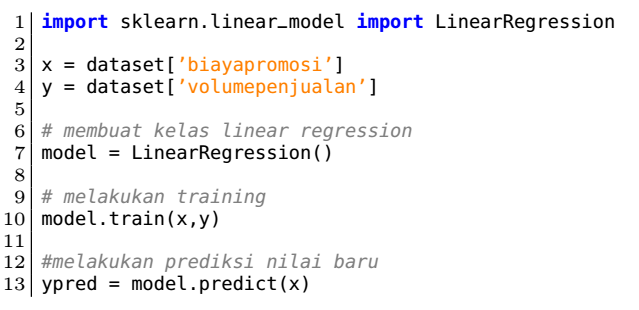
\includegraphics[scale=0.6]{bab4/code_analisislinearregression}   
	\caption{Kode contoh \textit{linear regression}}
	\label{fig:code_analisislinearregression} 
\end{figure} 


\section{Analisis Penerapan Polynomial Regression}
Berdasarkan penjelasan pada Landasan Teori Bab \ref{chap:teori} tentang \textit{Polynomial Regression}, maka diberikan contoh perhitungan prediksi menggunakan \textit{polynomial regression}. Terdapat \textit{dataset} dengan 2 variabel yaitu suhu ruangan dan jumlah cacat produksi.

\begin{table}[H]
\caption{Tabel dataset polinomial }
\centering
\begin{tabular}{|c|c|}
\hline 
Biaya Promosi (X) & Volume Penjualan (Y) \\ 
\hline 
12 & 56 \\ 
\hline 
14 & 62 \\ 
\hline 
13 & 60 \\ 
\hline 
12 & 61 \\ 
\hline 
15 & 65 \\ 
\hline 
13 & 66 \\ 
\hline 
14 & 60 \\ 
\hline 
15 & 63 \\ 
\hline 
13 & 65 \\ 
\hline 
14 & 62 \\ 
\hline 
\end{tabular} 
\label{tab:datasetpolynom}
\end{table}

Biaya promosi pada Tabel \ref{tab:datasetpolynom} merupakan variabel prediktor / independen (X). Volume penjualan pada Tabel \ref{tab:dataset} merupakan variabel dependen / respon (Y). Tujuan \textit{polynomial} adalah memprediksi volume penjualan berdasarkan biaya promosi yang dikeluarkan. Menggunakan persamaan \textit{polynomial regression}, maka perlu menghitung komponen untuk persamaan \eqref{eqref:hubunganpolinom} hubungan berupa $\sum x$ , $\sum y$ , $\sum x^2$ , $\sum x^3$ , $\sum x^4$ , $\sum xy$ dan $\sum x^2 y$ pada Tabel \ref{tab:tabelhubunganpolinomcontoh}.

\begin{table}[H]
\caption{perhitungan komponen matriks hubungan polinom orde 2}
\centering 
\begin{tabular}{|c|c|c|c|c|c|c|c|}
\hline 
no & x & y & $x^2$ & $x^3$ & $x^4$ & xy & $x^2 y$ \\ 
\hline 
1 & 12 & 56 & 144 & 1728 & 20736 & 672 & 9064 \\ 
\hline 
2 & 14 & 62 & 196 & 2744 & 48416 & 868 & 12152 \\ 
\hline 
3 & 13 & 60 & 169 & 2197 & 28561 & 780 & 10140 \\ 
\hline 
4 & 12 & 61 & 144 & 1728 & 20736 & 732 & 8784 \\ 
\hline 
5 & 15 & 65 & 225 & 3375 & 50625 & 975 & 14625 \\ 
\hline 
6 & 13 & 66 & 169 & 2197 & 28561 & 858 & 11154 \\ 
\hline 
7 & 14 & 60 & 196 & 2744 & 38416 & 840 & 11760 \\ 
\hline 
8 & 15 & 63 & 225 & 3375 & 50625 & 945 & 14175 \\ 
\hline 
9 & 13 & 65 & 169 & 2197 & 28561 & 845 & 10985 \\ 
\hline 
10 & 14 & 62 & 196 & 2744 & 38416 & 868 & 12152 \\ 
\hline 
$\sum  $ & 135 & 620 & 1833 & 25029 & 343653 & 8383 & 113991 \\ 
\hline 
\end{tabular} 
\label{tab:tabelhubunganpolinomcontoh}
\end{table}

Perhitungan Tabel \ref{tab:tabelhubunganpolinomcontoh} akan dimasukkan ke persamaan hubungan polinom.

\begin{displaymath}
		\begin{cases}
		   	(10)a_0 + (135) a_1 + (1833)a_2 &= 620 \\
		   		(135) a_0 + (1833)a_1 + (25049)a_2 &= 8383 \\
		   		(1833)a_0 + (25049)a_1 + (343653)a_2 &= 113991	   
		\end{cases}  
\end{displaymath} 

Menghitung koefisien a0,a1 dan a2 dapat menggunakan operasi matriks perkalian invers.
\begin{displaymath}
			\begin{bmatrix}
			10 & 135 & 1833 \\
			135  & 1833 & 25049 \\
			1833 & 25049 & 343653 
			\end{bmatrix}
			\begin{bmatrix}
			a0 \\ 
			a1 \\ 
			a2
			\end{bmatrix}
			=
			\begin{bmatrix}
				 620\\
				8383 \\
				 113991
			\end{bmatrix}
\end{displaymath}

Berdasarkan perhitungan matriks, maka didapatkan a0 = -67.96428571 , a1 = 18.11309524  dan a2 = -0.625. Hasil perhitungan tiap koefisien dapat dimasukkan pada persamaan \ref{eqref:persamaanpolinom} sehingga membentuk persamaan untuk menghitung volume penjualan (Y) menggunakan biaya promosi (X).


\begin{displaymath}
 Y = -67.96 + 18.11(Biaya Promosi) + (-0.63)(Biaya Promosi)^2 
\end{displaymath}


Menggunakan persamaan yang sudah diperoleh, maka prediksi volume penjualan (Y) menggunakan \textit{polynomial regression} dapat dihitung menggunakan biaya promosi. Berikut adalah  perbandingan antara volume penjualan asli (Y) dan volume penjualan prediksi \textit{polynomial regression} (\^{Y}) pada Tabel \ref{tab:perbandinganpolynomialregression}.

\begin{table}[H]
\caption{Perbandingan prediksi volume penjualan (Y) polynomial regression}
\centering
\begin{tabular}{|c|c|c|}
\hline 
Biaya Promosi (X) & Volume Penjualan (Y) & Prediksi Volume Penjualan (\^{Y})  \\ 
\hline 
12 & 56 & 59.39 \\ 
\hline 
14 & 62 & 63.11 \\ 
\hline 
13 & 60 & 61.88 \\ 
\hline 
12 & 61 & 59.39 \\ 
\hline 
15 & 65 & 63.10 \\ 
\hline 
13 & 66 & 61.88 \\ 
\hline 
14 & 60 & 63.11 \\ 
\hline 
15 & 63 & 63.10 \\ 
\hline 
13 & 65 & 61.88 \\ 
\hline 
14 & 62 & 63.11 \\ 
\hline 
\end{tabular} 
\label{tab:perbandinganpolynomialregression}
\end{table}

\textit{Library Scikit Learn} pada \textit{Python} menyediakan fungsi untuk melakukan prediksi menggunakan \textit{Polynomial Regression}. Kelas yang digunakan sama seperti \textit{Linear Regression}, tetapi ada modifikasi yaitu pengubahan variabel \textit{prediktor} untuk diubah sesuai dengan bentuk matriks koefisien untuk mendapatkan bentuk polinom dengan order sesuai \textit{input}. Gambar \ref{fig:code_analisispolynomialregression} adalah contoh potongan kode untuk melakukan prediksi menggunakan \textit{polynomial regression}. 


\begin{figure}[H]
	\centering  
	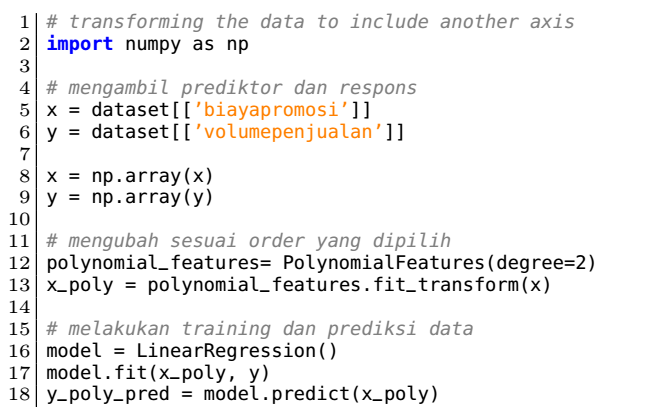
\includegraphics[scale=0.6]{bab4/code_analisispolynomialregression}   
	\caption{Kode contoh \textit{polynomial regression}}
	\label{fig:code_analisispolynomialregression} 
\end{figure} 

 

%\begin{lstlisting}[language=Python, caption=Library Polynomial Regression]
%# transforming the data to include another axis
%import numpy as np 
%
%# mengambil prediktor dan respons
%x = dataset[['biayapromosi']]
%y = dataset[['volumepenjualan']]
%
%x = np.array(x)
%y = np.array(y)
%
%# mengubah sesuai order yang dipilih
%polynomial_features= PolynomialFeatures(degree=2)
%x_poly = polynomial_features.fit_transform(x)
%
%# melakukan training dan prediksi data
%model = LinearRegression()
%model.fit(x_poly, y)
%y_poly_pred = model.predict(x_poly)
%
%\end{lstlisting}

Berdasarkan analisis mengenai penggunaan \textit{Linear Regression} dan \textit{Polynomial Regression}, Terdapat beberapa perbedaan yaitu kurva yang dihasilkan. Berikut adalah 2 gambar visualisasi kurva yang dihasilkan \textit{Linear} dan \textit{Polynomial Regression}.
\begin{figure}[H]
	\centering  
	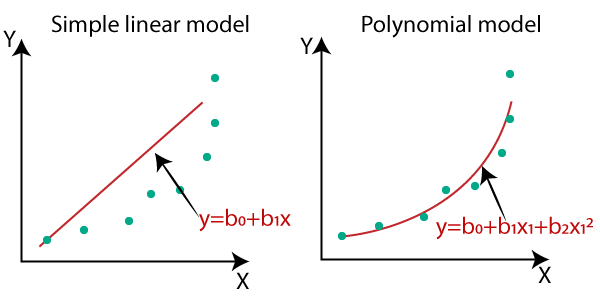
\includegraphics[scale=0.4]{bab3/kurvaregression}   
	\caption{Perbandingan kurva linear dan polinom}
	\label{fig:kurvaregression} 
\end{figure} 

Uraian Gambar \ref{fig:kurvaregression} di atas menjelaskan perbedaan kurva yang dihasilkan dari kedua algoritma. Masing-masing memiliki karakteristik yang dapat dicocokan berdasarkan sifat data yang digunakan. Selain itu, berikut adalah perbedaan yang dapat digunakan untuk memahami kedua algoritma \textit{Regression} yaitu : 

\begin{itemize}
\item \textit{Linear Regression} digunakan untuk korelasi data yang memiliki hubungan linear 
\item \textit{Linear Regression} dengan menggunakan 2 atau lebih prediktor dapat disebut dengan \textit{Multiple Linear Regression}
\item \textit{Polynomial Regression} digunakan untuk korelasi data yang memiliki hubungan non linear seperti eksponensial 
\item Pemilihan \textit{order} pada \textit{Polynomial Regression} dapat mempengaruhi seberapa \textit{fit} (cocok) \textit{model} prediksi yang dibuat berdasarkan data yang digunakan 
\item Pemilihan angka \textit{order} yang besar pada \textit{Polynomial Regression} dapat menyebabkan model prediksi yang dibuat menyebabkan \textit{overfit}. \textit{Overfit} adalah kondisi dimana model yang dibuat memiliki akurasi yang sangat baik terhadap data \textit{test} tetapi akan membuat prediksi terhadap data yang tidak terduga menjadi buruk. 
\end{itemize}

\section{Analisis Penerapan Evaluasi Regresi}
Hasil prediksi nilai yang diprediksi menggunakan \textit{Linear Regression} dan \textit{Polynomial Regression} dapat diukur seberapa akurat menggunakan \textit{Mean Squared Error (MSE)} dan \textit{Coefficient Determination} (R2). Berdasarkan hasil prediksi yang dijelaskan pada bagian prediksi \textit{Linear Regression} sebelumnya, berikut adalah perhitungan mengukur akurasi prediksi menggunakan persamaan \textit{Coefficient of Determination} yang akan ditunjukkan pada tabel di bawah.


\begin{table}[H]
\caption{Tabel perhitungan R2 berdasarkan contoh prediksi Linear Regression}
\centering
\begin{tabular}{|c|c|c|c|}
\hline 
Volume Penjualan ($Y$) & Prediksi Volume Penjualan ($\hat{Y}$) & $(Y-\hat{Y})^2$ & $(Y-\bar{Y})^2$ \\ 
\hline 
56 & 60.14 & 17.14 & 37.21 \\ 
\hline 
62 & 62.62 & 0.38 & 0.01 \\ 
\hline 
60 & 61.38 & 1.90 & 4.41 \\ 
\hline 
61 & 60.14 & 0.73 & 1.21 \\ 
\hline 
65 & 63.86 & 1.29 & 8.41 \\ 
\hline 
66 & 61.38 & 21.34 & 15.21 \\ 
\hline 
60 & 62.61 & 6.81 & 4.41 \\ 
\hline 
63 & 63.86 & 0.73 & 0.81 \\ 
\hline 
65 & 61.38 & 13.10 & 8.41 \\ 
\hline 
63 & 62.61 & 0.15 & 0.81 \\ 
\hline 
\multicolumn{4}{|c|}{•} \\ 
\hline 
\multicolumn{2}{|c|}{$\sum{}^{} Sum$} & 63.62 & 80.9 \\ 
\hline 
\multicolumn{3}{|c|}{Mean (Y)} & 62.1 \\ 
\hline 
\end{tabular} 
\label{tab:TabelPerhitunganR2}
\end{table}

Berdasarkan uraian tabel \ref{tab:TabelPerhitunganR2} di atas,nilai \textit{Coefficient Determination} dari prediksi Volume Penjualan menggunakan \textit{Linear Regression} dapat dihitung.

\begin{equation}
R2 = 1 - \frac{\sum{}^{}(y-\hat{y})^2}{ (y-\bar{y})^2}
\end{equation}

\begin{equation}
R2 = 1 - \frac{63.62}{90.9} = 0.21
\label{eqref:ContohRumusR2}
\end{equation}

Berdasarkan hasil persamaan \eqref{eqref:ContohRumusR2} di atas, evaluasi prediksi Volume Penjualan menggunakan \textit{Linear Regression} berdasarkan R2 adalah $0.21$. Nilai R2 adalah nilai yang berada diantara dari $0$ sampai $1.0$. Semakin tinggi nilainya semakin akurat prediksinya. Nilai R2 memberikan evaluasi adanya korelasi antara prediktor dan \textit{response} tetapi tidak terlalu kuat. Umumnya nilai prediksi yang bagus dan akurat adalah di atas $0.7$.

\textit{Library Scikit Learn} pada \textit{Python} menyediakan perhitungan \textit{Coefficient Determination}  pada \textit{Package} \textit{metrics} yaitu \textit{method} \textit{r2\textunderscore score(actual , pred)} yang menerima nilai asli dan nilai prediksi untuk dihitung nilai akurasi. Berikut adalah potongan kode \textit{r2\textunderscore score} yaitu : 

%\begin{lstlisting}[language=Python, caption=Library R2 Score]
%#asumsikan sudah dilakukan prediksi 
%# variabel nilai resonse asli = y
%# variabel nilai response prediksi model = ypred 
%from sklearn.metrics import r2_score 
%
%nilaiAkurasi = r2_score(y, ypred)
%
%\end{lstlisting}


\begin{figure}[H]
	\centering  
	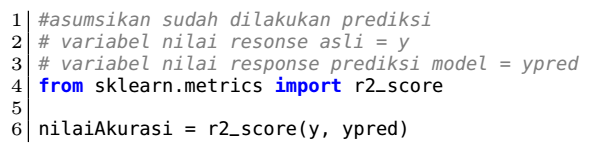
\includegraphics[scale=0.6]{bab4/code_evaluasiregresi}   
	\caption{Kode contoh \textit{evaluasi regresi}}
	\label{fig:code_evaluasiregresi} 
\end{figure}

\section{Analisis Penerapan K-NN}
Berdasarkan penjelasan pada Bab \ref{chap:teori} mengenai klasifikasi, \textit{K-NN} adalah algoritma \textit{classification} untuk menentukan label sebuah data. Akan diberikan contoh perhitungan menggunakan \textit{k-Nearest Neighbor} untuk memprediksi nilai kategori pada data baru. Berikut adalah contoh \textit{data set} yang digunakan sebagai \textit{training set} untuk membuat model \textit{k-Nearest Neighbor}.

\begin{table}[H]
\caption{Tabel dataset k-nearest neighbor}
\centering 
\begin{tabular}{|c|c|c|}
\hline 
x & y & kategori \\ 
\hline 
7 & 6 & Bad \\ 
\hline 
6 & 6 & Bad \\ 
\hline 
6 & 5 & Bad \\ 
\hline 
1 & 3 & Good \\ 
\hline 
2 & 4 & Good \\ 
\hline 
2 & 2 & Good \\ 
\hline 
\end{tabular} 
 \label{tab:datasetknn}
 \end{table}
 
 Tabel \ref{tab:datasetknn} berisi 2 variabel prediktor / independen yaitu x dan y. Kategori merupakan variabel respon / dependen. Diberikan sebuah data objek baru dengan x = 3 dan y = 5. Algoritma \textit{k-Nearest Neighbors}  memilih k tetangga terdekat.  Nilai k yang ditentukan adalah 3. Menggunakan \textit{euclidean distance}, berikut adalah perhitungan jarak setiap data pada \textit{data set}  dengan data baru. 
 
 \begin{table}[H]
  \caption{Tabel perhitungan euclidean distance dengan data baru}
 \centering
\begin{tabular}{|c|c|c|c|c|}
 \hline 
 x & y & kategori & euclidean distance dengan data baru & perhitungan \\ 
 \hline 
 7 & 6 & Bad & 4.12 & $\sqrt{(7-3)^2+(6-5)^2}$ \\ 
 \hline 
 6 & 6 & Bad & 3.16 & $\sqrt{(6-3)^2+(6-5)^2}$ \\ 
 \hline 
 6 & 5 & Bad & 3 & $\sqrt{(6-3)^2+(5-5)^2}$ \\ 
 \hline 
 1 & 3 & Good & 2.82 & $\sqrt{(1-3)^2+(3-5)^2}$ \\ 
 \hline 
 2 & 4 & Good & 1.41 & $\sqrt{(2-3)^2+(3-5)^2}$ \\ 
 \hline 
 2 & 2 & Good & 3.16 & $\sqrt{(2-3)^2+(2-5)^2}$ \\ 
 \hline 
 \end{tabular}  
 \label{tab:hitunganeuclideandistanceknn}
  \end{table}
  
Setelah menghitung setiap jarak dengan data baru, maka \textit{k-Nearest Neighbors} akan memilih tetangga terdekat sebanyak k. Karena nilai k adalah 3, maka akan dipilih kategori berdasarkan tiga tetangga dengan selisih jarak \textit{euclidean distance} minimum. Berikut adalah 3 tetangga terdekat dengan data baru pada Tabel \ref{tab:tabel3tetangga}.

\begin{table}[H]
\caption{Tabel 3 tetangga terdekat berdasarkan perhitungan euclidean distance}
\centering
\begin{tabular}{|c|c|c|c|}
\hline 
x & y & kategori & Jarak dengan data baru \\ 
\hline 
2 & 4 & Good & 1.41 \\ 
\hline 
1 & 3 & Good & 2.82 \\ 
\hline 
6 & 5 & Bad & 3 \\ 
\hline 
\end{tabular} 
\label{tab:tabel3tetangga}
 \end{table}

Tabel \ref{tab:tabel3tetangga} menunjukkan bahwa terdapat 3 tetangga terdekat. Algoritma \textit{k-Nearest Neighbors} akan menentukan kategori dari data baru berdasarkan jarak terdekat dan paling banyak. Pada 3 jarak terdekat, terdapat 2 kategori "Good" dan 1 kategori "Bad". Karena jumlah "Good" lebih banyak daripada "Bad", maka data baru akan memiliki kategori "Good". Melakukan evaluasi pada hasil prediksi menggunakan \textit{classification} menghitung \textit{accuracy}. \textit{Accuracy} dapat diperoleh dengan menghitung jumlah perbandingan prediksi yang benar dari semua data yang diprediksi.

\textit{Library Scikit Learn} pada \textit{Python} menyediakan fungsi untuk melakukan klasifikasi menggunakan K-NN yaitu \textit{package neighbors} kelas \textit{KNeighborsClassifier}. Prediksi label kelas menggunakan \textit{library} menerima sebuah \textit{input} yaitu \textit{n\textunderscore neighbors} yaitu jumlah tetangga terdekat yang menjadi penentu jumlah label terdekat. Berikut potongan kode \textit{K-NN} .



%\begin{lstlisting}[language=Python, caption=Library KNN]
%from sklearn.neighbors import KNeighborsClassifier
%
%#Buat model dgn jumlah neighbor = 2
%neighbor = 2
%kNN_model_iris = KNeighborsClassifier(n_neighbors=neighbor)
%
%#Train the model using the training sets
%kNN_model_iris.fit(x,y)
%
%#Predict the response for test dataset
%y_pred = kNN_model_iris.predict(x)
%\end{lstlisting}

\begin{figure}[H]
	\centering  
	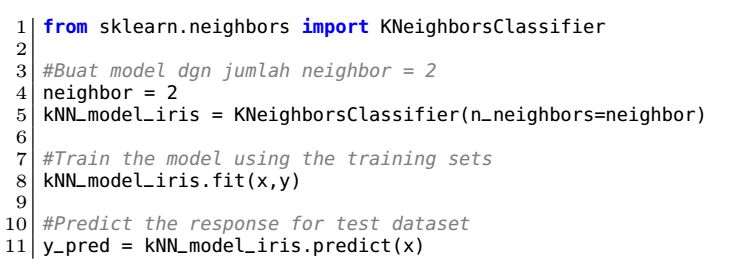
\includegraphics[scale=0.6]{bab4/code_analisisknn}   
	\caption{Kode contoh \textit{K-NN}}
	\label{fig:code_analisisknn} 
\end{figure} 

\section{Analisis Penerapan Evaluasi Klasifikasi}
Evaluasi klasifikasi yaitu adalah cara melakukan evaluasi apakah hasil prediksi yang dihasilkan akurat. Berdasarkan Landasan Teori tentang evaluasi Klasifikasi, berikut akan diberikan contoh dalam melakukan evaluasi klasifikasi. Diberikan \textit{dataset} nilai label asli dan hasil prediksi.


\begin{table}[H]
\caption{Tabel dataset evaluasi klasifikasi}
\centering
\begin{tabular}{|c|c|}
\hline 
Label Asli ($y$) & Label Prediksi ($\hat{y}$) \\ 
\hline 
GOOD & BAD \\ 
\hline 
GOOD & GOOD \\ 
\hline 
BAD & BAD \\ 
\hline 
BAD & BAD \\ 
\hline 
\end{tabular} 
\label{tab:tabelevaluasiklasifikasi}
\end{table}

Tabel \ref{tab:tabelevaluasiklasifikasi} di atas merupakan hasil perbandingan nilai label asli dan hasil label prediksi menggunakan klasifikasi. Terdapat 1 baris data yang tidak konsisten. Label asli dan label prediksinya tidak sesuai yang berarti prediksinya salah. Dari 4 observasi, terdapat 3 observasi yang prediksinya sesuai sehingga nilai evaluasinya adalah $0.75$. Gambar \ref{fig:code_analisisevaluasiklasifikasi} adalah contoh potongan kode untuk menghitung evaluasi klasifikasi.

%\begin{lstlisting}[language=Python, caption=Library Evaluasi Klasifikasi]
%from sklearn.neighbors import KNeighborsClassifier
%
%#Buat model dgn jumlah neighbor = 5
%neighbor = 5
%kNN_model_iris = KNeighborsClassifier(n_neighbors=neighbor)
%
%#Train the model using the training sets
%kNN_model_iris.fit(X_train, y_train)
%
%#Predict the response for test dataset
%y_pred = kNN_model_iris.predict(X_test)
%
%#Import scikit-learn metrics module for accuracy calculation
%from sklearn import metrics
%# Model Accuracy, how often is the classifier correct?
%print("Accuracy model klasifikasi Iris dgn neighbor = ",  neighbor, ": ",metrics.accuracy_score(y_test, y_pred))
%
%\end{lstlisting}


\begin{figure}[H]
	\centering  
	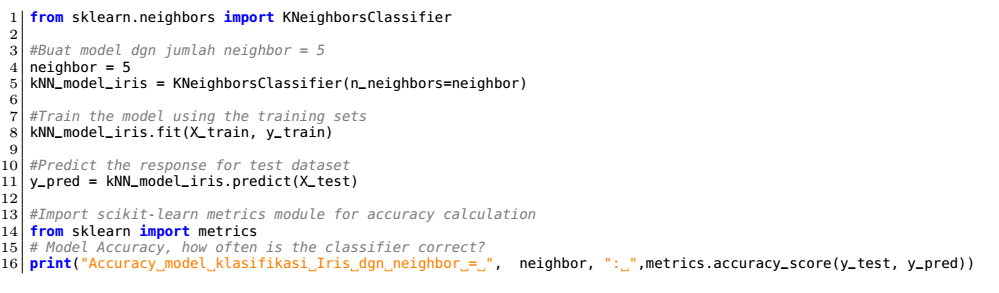
\includegraphics[scale=0.6]{bab4/code_analisisevaluasiklasifikasi}   
	\caption{Kode contoh evaluasi klasifikasi}
	\label{fig:code_analisisevaluasiklasifikasi} 
\end{figure} 

\section{Analisis Penerapan K-Means}
Berdasarkan Landasan Teori Bab \ref{chap:teori} tentang algoritma \textit{clustering}, \textit{K-Means} adalah cara untuk mengelompokkan data. Diberikan sebuah contoh perhitungan \textit{k-Means} untuk menentukan kelompok data. Berikut adalah contoh \textit{data set} nilai yang digunakan.

\begin{table}[H]
\caption{Tabel dataset k-Means}
\centering
\begin{tabular}{|c|c|c|c|}
\hline 
Nama & UTS & ART & UAS \\ 
\hline 
Jonathan & 75 & 40 & 95 \\ 
\hline 
James & 90 & 95 & 100 \\ 
\hline 
Pedro & 55 & 90 & 75 \\ 
\hline 
Luna & 85 & 65 & 85 \\ 
\hline 
Harry & 85 & 80 & 80 \\ 
\hline 
Chloe & 55 & 50 & 51 \\ 
\hline 
\end{tabular} 
\label{tab:datasetkmeans}
\end{table}

Tabel \ref{tab:datasetkmeans} memiliki informasi  / atribut berupa nilai UTS,ART dan UAS. K atau jumlah \textit{cluster} yang ditentukan adalah K=2. Titik awal \textit{centroid} yaitu c1 dan c2. Sesuai dengan cara kerja \textit{K-Means}, titik \textit{Centroid} diinisialisasi secara \textit{random} yaitu : 

\begin{itemize}
\item c1 : UTS(80) , ART(80),UAS(80)
\item c2 : UAS(50) , ART(50), UAS(50)
\end{itemize}

Berikut adalah perhitungan tiap data objek dengan menggunakan \textit{euclidean distance} pada persamaan \eqref{eqref:euclideandistance}.

\begin{table}[H]
\caption{Tabel perhitungan k-Means iterasi ke-1}
\centering
\scalebox{0.8}{
\begin{tabular}{|c|c|c|c|c|c|c|}
\hline 
Nama & UTS & ART & UAS & Dist(data(i),c1) & Dist(data(i),c2) & Kelompok \\ 
\hline 
Jonathan & 75 & 40 & 95 & $43.01$ &  $  53.44$ & c1 \\ 
\hline 
James & 90 & 95 & 100 &  $ 26.92$ & $ 78.26$ & c1 \\ 
\hline 
Pedro & 55 & 90 & 75 & $ 27.38$ & $ 47.43$  & c1 \\ 
\hline 
Luna & 85 & 65 & 85 &  $ 16.58$ & $ 51.72$ & c1 \\ 
\hline 
Harry & 85 & 80 & 80 &  $5$ & $ 55$ & c1 \\ 
\hline 
Chloe & 55 & 50 & 51 & $ 48.64$ &$5.09$ & c2 \\ 
\hline 
\end{tabular}}
\label{tab:kmeansiterasi1}
\end{table} 

Tabel \ref{tab:kmeansiterasi1} menunjukkan perhitungan iterasi pertama untuk mendapatkan kelompok tiap data objek. Titik \textit{centroid} akan diubah dengan menghitung rata-rata atribut tiap anggota kelompok yang baru ditentukan pada Tabel \ref{tab:centroid1}.

\begin{table}[H]
\caption{Tabel perubahan centroid iterasi 2}
\centering
\begin{tabular}{|c|c|c|c|}
\hline 
Nama & UTS & ART & UAS \\ 
\hline 
c1 & $\frac{(75+90+55+85+85)}{5} =  78$ & $ \frac{(40+95+90+65+80)}{5} = 74$ & $\frac{(95+100+75+85+80)}{5} = 87$ \\ 
\hline 
c2 & 55 & 50 & 51 \\ 
\hline 
\end{tabular} 
\label{tab:centroid1}
\end{table}

Setelah titik \textit{centroid} berubah, maka perhitungan tiap data objek dengan \textit{centroid} yang baru akan dilakukan.

\begin{table}[H]
\caption{Tabel perhitungan k-Means iterasi ke-2}
\centering
\begin{tabular}{|c|c|c|c|c|c|c|}
\hline 
Nama & UTS & ART & UAS & dist(c1) & dist(c2) & kelompok \\ 
\hline 
Jonathan & 75 & 40 & 95 & 35.05 & 49.35 & c1 \\ 
\hline 
James & 90 & 95 & 100 & 27.45 & 75.17 & c1 \\ 
\hline 
Pedro & 55 & 90 & 75 & 30.47 & 46.64 & c1 \\ 
\hline 
Luna & 85 & 65 & 85 & 11.57 & 51.39 & c1 \\ 
\hline 
Harry & 85 & 80 & 80 & 11.57 & 51.39 & c1 \\ 
\hline 
Chloe & 55 & 50 & 51 & 49 & 0 & c2 \\ 
\hline 
\end{tabular} 
\label{tab:kmeansiterasi2}
\end{table}
Karena pada Tabel \ref{tab:kmeansiterasi2} tiap data objek tidak berpindah ke \textit{cluster} lain, sehingga \textit{centroid} tidak perlu hitung kembali karena sudah konvergen.

\textit{Library Scikit Learn} pada \textit{Python} menyediakan fungsi untuk melakukan \textit{clustering K-Means} menggunakan \textit{package cluster} yaitu kelas \textit{KMeans}. Kelas \textit{KMeans} dapat memanggil fungsi \textit{fit} dengan parameter \textit{n\textunderscore cluster} yaitu jumlah kelompok yang ingin dibuat. Gambar \ref{fig:code_analisisclustering_kmeans} adalah potongan kode untuk melakukan \textit{clustering} dengan \textit{K-Means}.

%\begin{lstlisting}[language=Python, caption=Library K-Means]
%#Clustering dgn k-Means
%from sklearn.cluster import KMeans
%
%#Lakukan clustering (fit) dgn jumlah cluster = 3
%kmeans_model = KMeans(n_clusters=3, random_state=0).fit(X)
%
%#Print label cluster pada tiap rekord/objek
%kmeans_model.labels_
%
%#Print centroid (cluster centers)
%kmeans_model.cluster_centers_
%\end{lstlisting} 


\begin{figure}[H]
	\centering  
	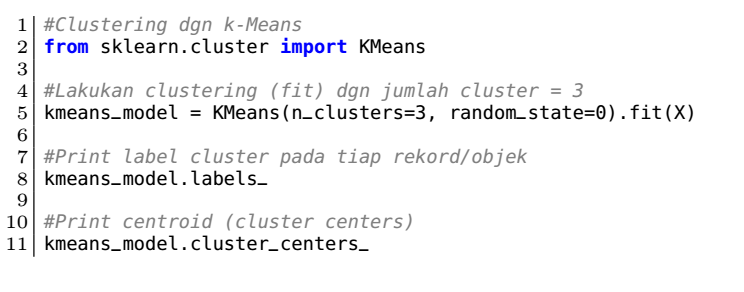
\includegraphics[scale=0.6]{bab4/code_analisisclustering_kmeans}   
	\caption{Kode contoh \textit{clustering K-Means}}
	\label{fig:code_analisisclustering_kmeans} 
\end{figure} 

\section{Analisis Penerapan Agglomerative}
Berdasarkan penjelasan Landasan Teori Bab \ref{chap:teori} tentang \textit{Agglomerative Clustering}, diberikan contoh perhitungan cara memprediksi sebuah nilai dengan \textit{Agglomerative Clustering}. Berikut adalah sebuah \textit{dataset} yang digunakan.

\begin{table}[H]
\caption{Tabel dataset perhitungan agglomerative}
\centering
\begin{tabular}{|c|c|c|c|}
\hline 
Nama & UTS & ART & UAS \\ 
\hline 
Jonathan & 74 & 40 & 95 \\ 
\hline 
James & 90 & 95 & 100 \\ 
\hline 
Pedro & 55 & 90 & 75 \\ 
\hline 
Luna & 85 & 65 & 85 \\ 
\hline 
\end{tabular} 
\label{tab:datasetagglomerative}
\end{table} 
Tabel \ref{tab:datasetagglomerative} berisi komponen nilai tiap siswa yaitu UTS,ART dan UAS. Berikut adalah perhitungan jarak tiap data objek menggunakan \textit{euclidean distance}.

\begin{table}[H]
\caption{Tabel perhitungan euclidean distance iterasi pertama}
\centering
\begin{tabular}{|c|c|c|c|c|}
\hline 
& Jonathan & James & Pedro & Luna \\ 
\hline 
Jonathan & 0 &  &  &  \\ 
\hline 
James & $\sqrt{(75-90)^2 + (40-95)^2 + (95-100)^2} = 57.22$ & 0 &  &  \\ 
\hline 
Pedro & $\sqrt{(75-55)^2 + (40-90)^2 + (95-75)^2} = 57.44$ &  43.4 & 0 &  \\ 
\hline 
Luna & \cellcolor{yellow!25}  28.72 &  33.91 & 40.31 & 0 \\ 
\hline 
\end{tabular} 
\label{tab:agglomerativeiterasi1}
\end{table}

Tabel \ref{tab:agglomerativeiterasi1} berisi perhitungan jarak tiap data objek. Karena jarak Jonathan dan Luna paling kecil, maka akan dikelompokkan menjadi satu \textit{cluster} yang sama yaitu c1. Satu \textit{cluster} yang terdiri dari beberapa titik dapat dihitung berdasarkan rata-rata tiap atribut sehingga isi \textit{data set} berubah. 



\begin{table}[H]
\caption{Tabel perubahan nilai cluster iterasi 1}
\centering 
\begin{tabular}{|c|c|c|c|}
\hline 
\textbf{Euclidean Distance} & Jonathan,Luna & James & Pedro \\ 
\hline 
Jonathan,Luna & $75+85/2 = 80 $ & $40+65/2 = 52.5$ & $95+85/2 = 85$ \\ 
\hline 
James & 90 & 95 & 100 \\ 
\hline 
Pedro & 55 & 80 & 75 \\ 
\hline 
\end{tabular} 
\label{tab:perubahandatasetagglo1}
\end{table}

Tabel \ref{tab:perubahandatasetagglo1} menunjukkan perubahan titik tengah \textit{cluster} berasal dari rata-rata atribut Jonathan dan Luna. Iterasi selanjutnya akan menghitung jarak antara tiap titik untuk mencari jarak terpendek.

\begin{table}[H]
\caption{Tabel perhitungan euclidean distance iterasi kedua }
\centering
\begin{tabular}{|c|c|c|c|}
\hline 
\textbf{Euclidean Distance} & Jonathan,Luna (c1) & James & Pedro \\ 
\hline 
Jonathan,Luna (c1) & 0 & & \\ 
\hline 
James & 44.79 & 0 &  \\ 
\hline 
Pedro & \cellcolor{yellow!25} 40.07 & 45.55 & 0 \\ 
\hline 
\end{tabular} 
\label{tab:agglomerativeiterasi2}
\end{table}

Tabel \ref{tab:agglomerativeiterasi2} menunjukkan bahwa jarak antara c1 (Jonathan,Luna) dan Pedro memiliki jarak terpendek sehingga dikelompokkan menjadi satu \textit{cluster}. Setelah Pedro digabungkan dengan c1 menjadi c2, maka titik tengah dari c2 (Jonathan,Luna,Pedro) berubah.



\begin{table}[H]
\caption{Tabel perubahan nilai cluster iterasi 2}
\centering
\begin{tabular}{|c|c|c|c|}
\hline 
 & UTS & ART & UAS \\ 
\hline 
c2 (Jonathan,Luna, Pedro) & $(80+55)/2 = 67.5$ & $(52.55+80)/2 = 66.25$ & $(90+75)/2 = 82.5$ \\ 
\hline 
James & 90 & 95 & 100 \\ 
\hline 
\end{tabular} 
\label{tab:perubahandatasetagglo2}
\end{table} 

Tabel \ref{tab:perubahandatasetagglo2} menunjukkan bahwa tinggal terdapat 2 data objek yaitu \textit{cluster}
c2 dan James. Kedua data objek dapat digabung langsung tanpa harus menghitung jarak menjadi c3 (Jonathan, James ,Pedro, Luna). Visualisasi \textit{agglomerative clustering} dapat menggunakan dendogram. 


\begin{figure}[H]
	\centering  
	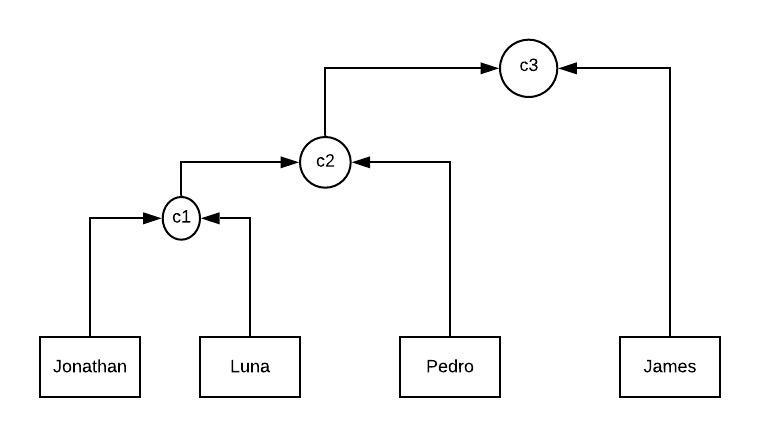
\includegraphics[scale=0.7]{bab2/dendogramcontoh}   		
	\caption{Dendogram example}
	\label{ref:dendogramcontoh} 
\end{figure} 



\textit{Library Scikit Learn} pada \textit{Python} menyediakan fungsi untuk melakukan \textit{clustering} menggunakan \textit{Agglomerative}. Memanggil \textit{package cluster} dan kelas \textit{AgglomerativeClustering} untuk melakukan \textit{clustering} membutuhkan 1 parameter yaitu \textit{n\textunderscore clusters} yaitu jumlah \textit{cluster} yang ingin dihasilkan dari \textit{clustering}. Berikut adalah potongan kode yang digunakan yaitu : 
%
%\begin{lstlisting}[language=Python, caption=Library Agglomerative Clustering]
%#Clustering dgn Agglomeratives
%from sklearn.cluster import AgglomerativeClustering
%#Lakukan clustering (fit) dgn jumlah cluster = 3
%agglo_model = AgglomerativeClustering(n_clusters=3).fit(X)
%#Print label cluster pada tiap rekord/objek
%agglo_model.labels_
%\end{lstlisting} 

\begin{figure}[H]
	\centering  
	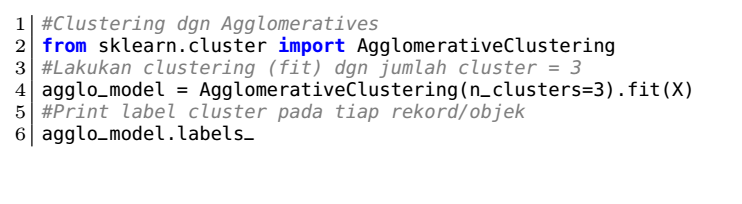
\includegraphics[scale=0.6]{bab4/code_analisisclustering_agglo}   
	\caption{Kode contoh \textit{agglomerative clustering}}
	\label{fig:code_analisisclustering_agglo} 
\end{figure} 

\section{Analisis Penerapan Evaluasi Clustering} 
Berdasarkan Landasan Teori pada Bab \ref{chap:teori} mengenai evaluasi \textit{clustering} terdapat 
salah satu teknik evaluasi \textit{clustering} yaitu \textit{silhouette plot}. Berikut diberikan \textit{dataset} contoh. 

\begin{table}[H]
\centering
\begin{tabular}{|c|c|c|}
\hline 
Murid & Nilai & Kelompok \\ 
\hline 
A & 20 & C1 \\ 
\hline 
B & 30 & C1 \\ 
\hline 
C & 40 & C1 \\ 
\hline 
D & 70 & C2 \\ 
\hline 
E & 75 & C2 \\ 
\hline 
F & 90 & C3 \\ 
\hline 
G & 95 & C3 \\ 
\hline 
H & 100 & C3 \\ 
\hline 
\end{tabular} 
\caption{Tabel dataset contoh yang akan di evaluasi}
\label{tab:datasetevaluasiclustering}
\end{table}

Tabel \ref{tab:datasetevaluasiclustering} adalah contoh hasil  \textit{clustering} untuk mengelompokkan siswa berdasarkan nilai. Pada tahap ini akan dihitung nilai \textit{silhouette plot} dari murid "A" untuk mengukur kualitas \textit{cluster}.

\begin{equation}
 S(i) = \frac{(b(i)-a(i))}{max(a(i),b(i))}
 \label{eqref:contohsilhouetteplot}
\end{equation}

Persamaan \ref{eqref:contohsilhouetteplot} dapat digunakan untuk menghitung kualitas \textit{cluster}. Untuk menghitung \textit{silhouette plot} dari murid "A" / S(a), dibutuhkan nilai a dan b. Nilai $a(i)$ adalah rata-rata jarak murid "A" ke murid lain pada \textit{cluster} yang sama. Nilai $b(i)$ adalah rata-rata jarak murid "A" ke tetangga pada \textit{cluster} lain.

\begin{equation}
\label{eqref:contohperhitungansilhouetteplot}
\begin{split}
b(i) & = (dist(A,B) + dist(A,C)) / 2 \\
b(i) & = (dist(A,D) + dist(A,F)) / 2 \\
S(A)& = \frac{b(i)-a(i)}{max(b(i),a(i))} \\
 S(A) & = \frac{(60-15)}{max(60,15)} = 0.75
\end{split}
\end{equation}

Persamaan \ref{eqref:contohperhitungansilhouetteplot} adalah contoh hasil perhitungan untuk evaluasi \textit{cluster} pada titik "A". Nilai \textit{silhouette} adalah nilai yang memiliki rentang $0.0$ sampai $1.0$. Semakin tinggi nilai \textit{silhouette} maka semakin baik sebuah \textit{cluster}.
\textit{Library Scikit Learn} pada \textit{Python} menyediakan fungsi untuk menghitung hasil \textit{clustering} menggunakan \textit{silhouette plot}. Gambar \ref{fig:code_analisisevaluasiclustering} adalah contoh kode untuk menghitung \textit{silhouette plot}.

%\begin{lstlisting}[language=Python, caption=Library Evaluasi Clustering]
%from sklearn.metrics import silhouette_score 
%
%clusterer = KMeans(n_clusters=n_clusters)
%preds = clusterer.fit_predict(df)
%score = silhouette_score(df, preds)
%\end{lstlisting}

\begin{figure}[H]
	\centering  
	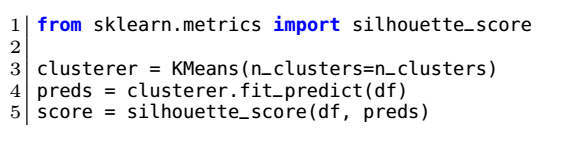
\includegraphics[scale=0.6]{bab4/code_analisisevaluasiclustering}   
	\caption{Kode contoh evaluasi clustering}
	\label{fig:code_analisisevaluasiclustering} 
\end{figure} 

\section{Analisis Visualisasi Data}
Visualisasi Data berdasarkan Landasan Teori Bab \ref{chap:teori} merupakan cara untuk merepresentasikan kumpulan data dalam bentuk gambar agar membantu memudahkan dalam melakukan analisis. Selain dari fungsi visualisasi, visualisasi data dapat dibagi berdasarkan dimensi data yang ditampilkan. \textit{Histogram} dan \textit{Boxplot} dapat digunakan untuk menampilkan data satu dimensi. Berikut diberikan contoh \textit{dataset} yang akan digunakan untuk melakukan visualisasi.


\begin{table}[H]
\caption{Tabel dataset analisis visualisasi}
\centering
\begin{tabular}{|c|c|}
  \hline 
  Nama Pasien & Umur Pasien \\ 
  \hline 
  Hashrul & 21 \\ 
  \hline 
  Giovanny & 22 \\ 
  \hline 
  Rasyif & 21 \\ 
  \hline 
  Syafira & 20 \\ 
  \hline 
  Nouval & 52 \\ 
  \hline 
  Alit & 30 \\ 
  \hline 
  Timoti & 60 \\ 
  \hline 
  \end{tabular}   
\label{tab:analisisvisualisasi}
\end{table}

Tabel \ref{tab:analisisvisualisasi} di atas merupakan contoh kumpulan data pasien beserta umurnya. Dengan visualisasi data, analisis untuk melihat persebaran pasien berdasarkan umur akan lebih mudah dengan \textit{Histogram} dan \textit{Boxplot}. Berikut adalah hasil dari kedua visualisasi yang dibuat.



\begin{figure}[H]
	\centering  
	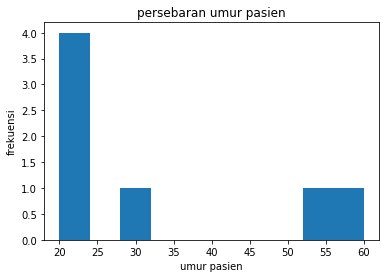
\includegraphics[scale=0.8]{bab3/histogramanalisis}    
	\caption{Contoh Analisis Histogram }
	\label{fig:histogramanalisis}
\end{figure} 


\begin{figure}[H]
	\centering  
	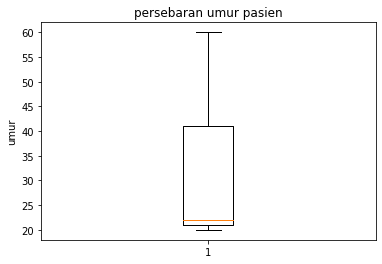
\includegraphics[scale=0.8]{bab3/boxplotanalisis}   
	\caption{Contoh Analisis Boxplot }
	\label{fig:boxplotanalisis} 
\end{figure} 


Gambar \ref{fig:histogramanalisis} dan \ref{fig:boxplotanalisis} merupakan hasil visualisasi dari \textit{dataset} yang sudah dijelaskan sebelumnya. Berdasarkan \textit{histogram}, dapat diidentifikasi kelompok umur mana yang paling banyak menjadi pasien. Berdasarkan \textit{boxplot} yang dihasilkan, dapat dideteksi nilai maksimum, minimum , Q1,Q2 dan Q3 dari data pasien. \textit{Library Matplotlib} pada \textit{Python} menyediakan fungsi untuk melakukan visualisasi seperti \textit{histogram} dan \textit{boxplot}. Gambar \ref{fig:code_analisisvisualisasi} adalah contoh potongan kode untuk melakukan visualisasi.


%\begin{lstlisting}[language=Python, caption=Library Visualisasi Data]
%import matplotlib.pyplot as plt 
%import pandas as pd 
%
%dataset = pd.read_csv('umurdataset.csv')
%
%#visualisasi menggunakan histogram
%plt.title('persebaran umur pasien') 
%plt.xlabel('umur pasien') 
%plt.ylabel('frekuensi')
%plt.hist(dataset.umur)
%plt.show()
%plt.clf()
%
%# visualisasi menggunakan boxplot
%plt.title('persebaran umur pasien') 
%plt.ylabel('umur') 
%plt.boxplot(dataset.umur)
%\end{lstlisting}

\begin{figure}[H]
	\centering  
	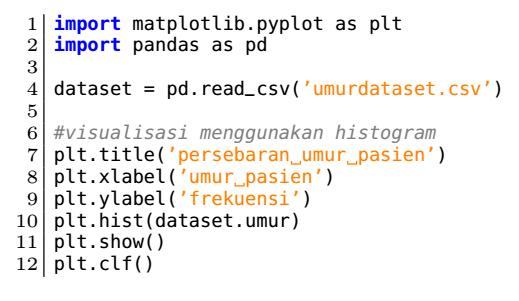
\includegraphics[scale=0.8]{bab4/code_analisisvisualisasi}   
	\caption{Kode contoh visualisasi }
	\label{fig:code_analisisvisualisasi} 
\end{figure} 




\section{Analisis Web Scrapping}
\label{chap:analisiswebscraping}
Penggunaan \textit{Web Scrapping} salah satunya adalah dengan menggunakan perangkat lunak yang memiliki fitur untuk melakukan \textit{Web Scrapping}. \textit{Octoparse} adalah perangkat lunak dengan antarmuka yang dapat mengambil sekumpulan elemen serupa pada sekumpulan \textit{web page}. Perangkat lunak ini sudah memiliki tampilan antarmuka sehingga lebih mudah untuk digunakan berikut adalah tampilan perangkat lunak dari \textit{octoparse}. Salah satu perangkat lunak yang akan digunakan pada penelitian ini adalah \textit{Octoparse}. Berikut adalah ilustrasi langkah \textit{Scrapping} menggunakan \textit{octoparse} dalam bentuk \textit{flowchart} pada Gambar \ref{fig:flowchartoctoparse}.


\begin{figure}[H]
	\centering  
	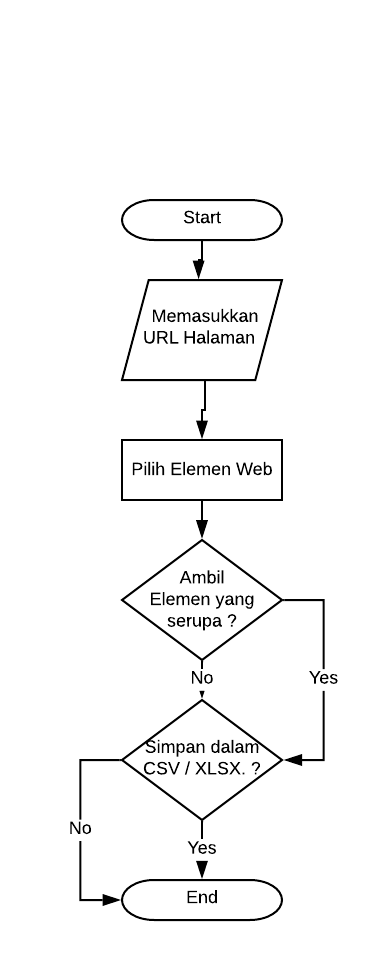
\includegraphics[scale=0.7]{bab3/flowchartoctoparse}   
	\caption{Flowchart Octoparse}
	\label{fig:flowchartoctoparse} 
\end{figure} 


\begin{figure}[H]
	\centering  
	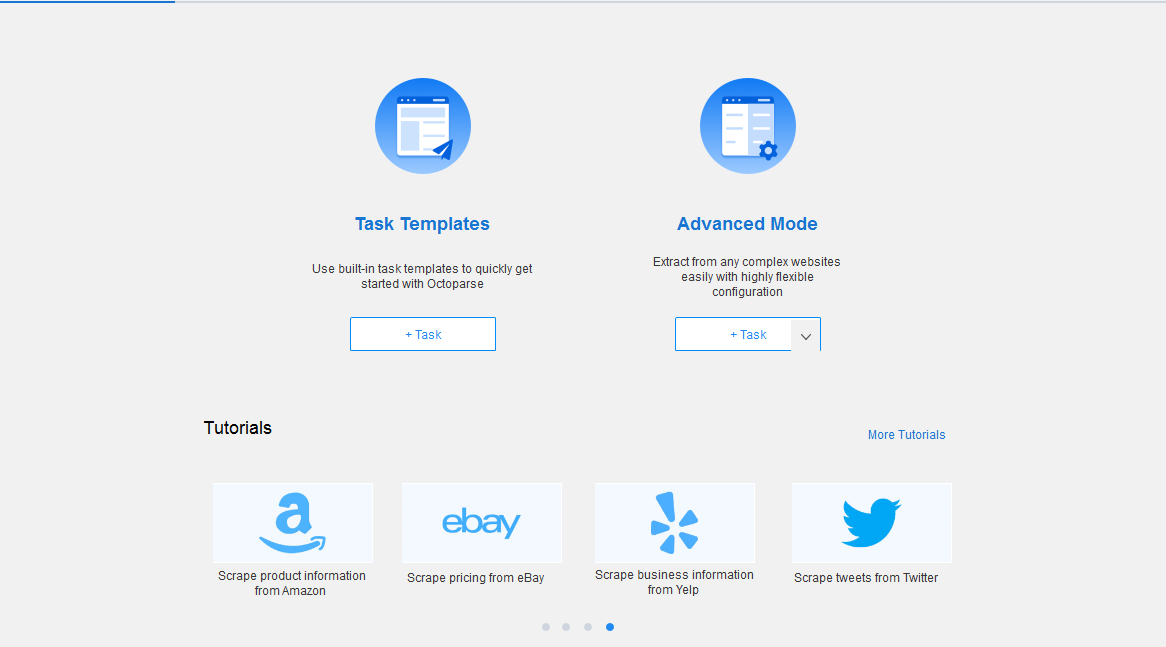
\includegraphics[scale=0.4]{bab3/tampilanoctoparse}   
	\caption{Tampilan utama Octoparse}
	\label{fig:tampilanoctoparse} 
\end{figure} 

Gambar \ref{fig:tampilanoctoparse} adalah tampilan utama dari \textit{Octoparse}. Diberikan contoh ilustrasi dalam melakukan \textit{scrapping} hasil pencarian situs \textit{google} dengan \textit{keyword digimon} untuk mengambil judul halaman pada pencarian.

\begin{figure}[H]
	\centering  
	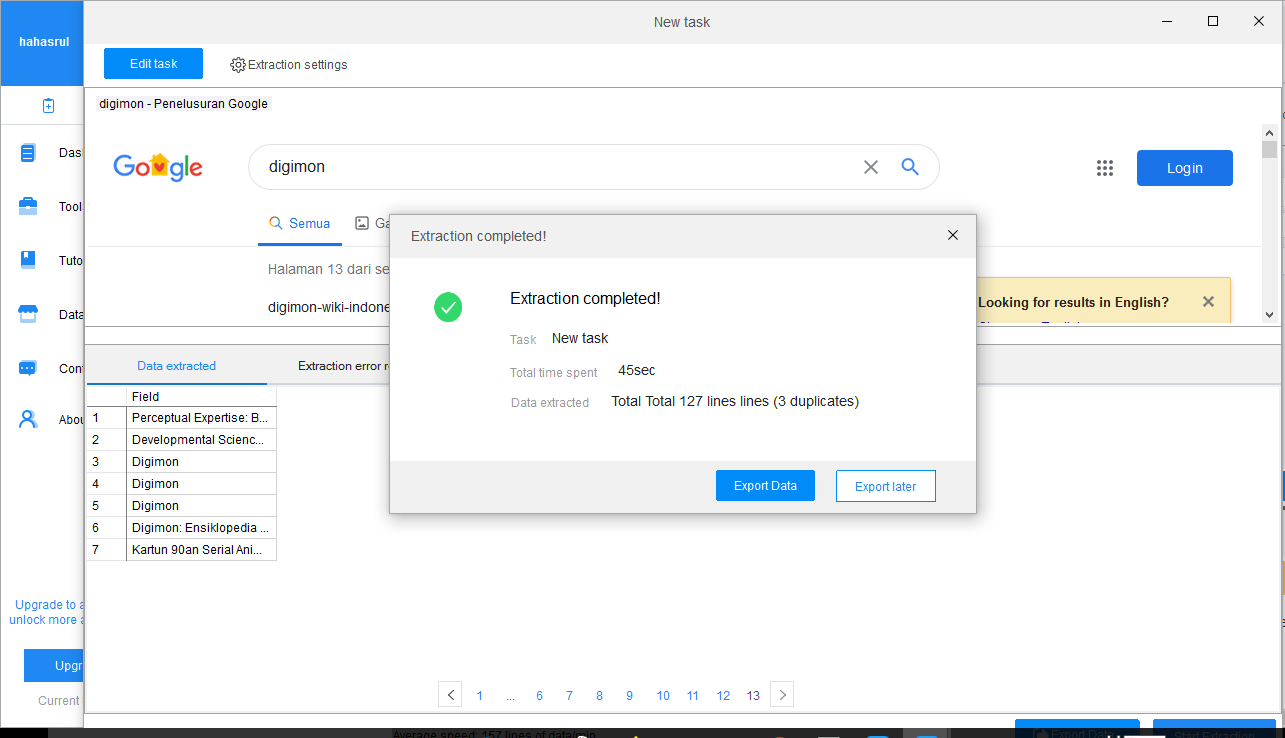
\includegraphics[scale=0.4]{bab3/scrapoctoparse}    
	\caption{Tampilan scrapping pada Octoparse}
	\label{fig:hasiloctoparse}
\end{figure} 

\textit{Output} dari \textit{Scrapping} sesuai Gambar \ref{fig:hasiloctoparse} berupa data tabel yang dapat disimpan dalam beberapa bentuk seperti CSV , Excel dan JSON. Hasil \textit{scrapping} serupa akan digunakan pada penelitian untuk melakukan \textit{data collection} agar analisis tambahan dapat dilakukan. 
